%!TEX root = ../BUSystematics.tex

\graphicspath{{Body/Figures/Gain/IFG/60h/Amplitude/}{Body/Figures/Gain/IFG/60h/Amplitude-With-AdHoc/}{Body/Figures/Gain/IFG/60h/Lifetime/}{Body/Figures/Gain/IFG/9d/Lifetime/}}

\section{Gain Systematic Errors}



\cite{GainElog}



-Describe generalities of gain effects here



- need to compare R vs T method results
- need to reference the errors used for the amplitude and the lifetime - hit weighted numbers David came up with for some datasets, and standard errors for the other datasets with the fixed tau ltdp
-record those errors into my table so people know exactly what they are
- describe the reasoning for the range for the linear fit in the lifetime case - perhaps include figures from other datasets showing the behavior
- point out that these two errors are highly correlated but I'm being very conservative and adding them in quadrature
- mention STDP as the results from with vs without the effect - reiterate that with my randomization scheme I don't have to worry about the statistics part as much, briefly mention that I don't have the ability to scan over the effect since I do things at the histogram level - do mention that I use Aaron's gain corrector module to make the trees...
- decide what I want to do for the ad hoc gain scan and then explain those results, include relevant plots, include updated plots for the IFG scan showing consistency with 1 afteer I have done so





\subsection{IFG Amplitude}


The systematic error due to the IFG amplitude was determined by 




\begin{figure}[h]
\centering
    \begin{subfigure}[t]{0.45\textwidth}
        \centering
        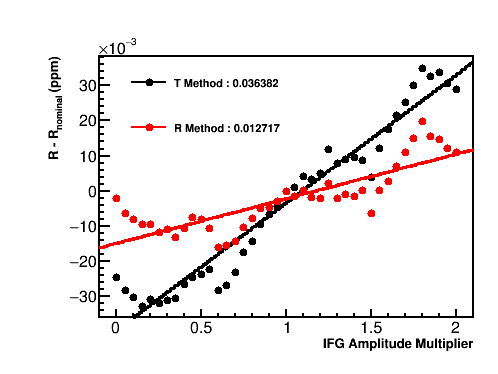
\includegraphics[width=\textwidth]{IFG_Amplitude_Compare_R}
        \caption{}
    \end{subfigure}% %you need this % here to add spacing between subfigures
    \hspace{1cm}
    \begin{subfigure}[t]{0.45\textwidth}
        \centering
        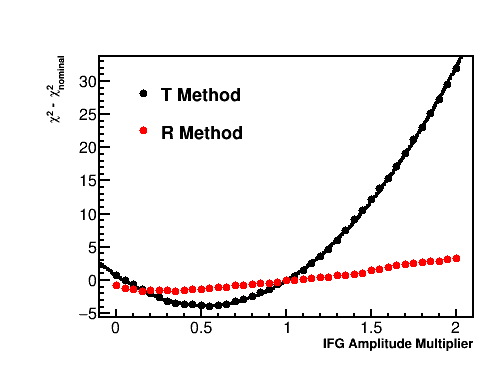
\includegraphics[width=\textwidth]{IFG_Amplitude_Compare_Chisq.png}
        \caption{}
    \end{subfigure}
\caption[Systematic error due to]{Systematic error due to. Data are from the 60h dataset.}
\label{fig:IFGAmpscan}
\end{figure}




\begin{table}
\centering
\renewcommand{\arraystretch}{1.2}
\begin{tabularx}{0.65\linewidth}{@{\extracolsep{\fill}}XYY}
  \hline
    \multicolumn{3}{c}{\textbf{Systematic Error due to}} \\
  \hline\hline
    Dataset & \thead{T-Method} & \thead{R-Method} \\
  \hline
    60h & 0.0 & 0.0 \\
    HighKick & 0.0 & 0.0 \\
    9d & 0.0 & 0.0 \\ 
    Endgame & 0.0 & 0.0 \\
  \hline
\end{tabularx}
\caption[Systematic error due to]{Systematic error due to. Units are in ppb.}
\label{tab:systematicError_}
\end{table}




\subsection{IFG Time Constant}



\begin{figure}[h]
\centering
    \begin{subfigure}[t]{0.45\textwidth}
        \centering
        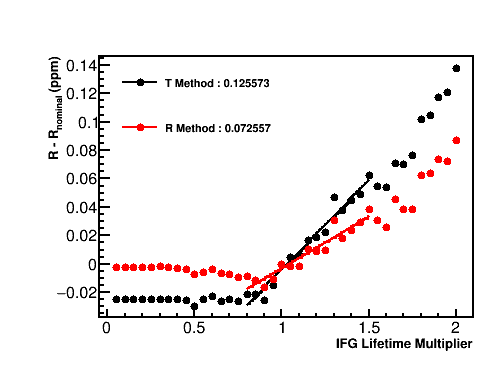
\includegraphics[width=\textwidth]{IFG_Lifetime_Compare_R}
        \caption{}
    \end{subfigure}% %you need this % here to add spacing between subfigures
    \hspace{1cm}
    \begin{subfigure}[t]{0.45\textwidth}
        \centering
        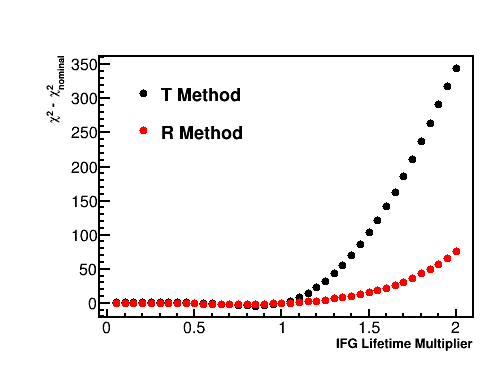
\includegraphics[width=\textwidth]{IFG_Lifetime_Compare_Chisq.png}
        \caption{}
    \end{subfigure}
\caption[Systematic error due to]{Systematic error due to. Data are from the 60h dataset.}
\label{fig:IFGAmpscan}
\end{figure}






\begin{table}
\centering
\renewcommand{\arraystretch}{1.2}
\begin{tabularx}{0.65\linewidth}{@{\extracolsep{\fill}}XYY}
  \hline
    \multicolumn{3}{c}{\textbf{Systematic Error due to}} \\
  \hline\hline
    Dataset & \thead{T-Method} & \thead{R-Method} \\
  \hline
    60h & 0.0 & 0.0 \\
    HighKick & 0.0 & 0.0 \\
    9d & 0.0 & 0.0 \\ 
    Endgame & 0.0 & 0.0 \\
  \hline
\end{tabularx}
\caption[Systematic error due to]{Systematic error due to. Units are in ppb.}
\label{tab:systematicError_}
\end{table}





\subsection{STDP}


- turned it on and off 



\begin{table}
\centering
\renewcommand{\arraystretch}{1.2}
\begin{tabularx}{0.65\linewidth}{@{\extracolsep{\fill}}XYY}
  \hline
    \multicolumn{3}{c}{\textbf{Systematic Error due to}} \\
  \hline\hline
    Dataset & \thead{T-Method} & \thead{R-Method} \\
  \hline
    60h & 0.0 & 0.0 \\
    HighKick & 0.0 & 0.0 \\
    9d & 0.0 & 0.0 \\ 
    Endgame & 0.0 & 0.0 \\
  \hline
\end{tabularx}
\caption[Systematic error due to]{Systematic error due to. Units are in ppb.}
\label{tab:systematicError_}
\end{table}







\subsection{Residual Gain Variation}

\begin{table}
\centering
\renewcommand{\arraystretch}{1.2}
\begin{tabularx}{0.65\linewidth}{@{\extracolsep{\fill}}XYY}
  \hline
    \multicolumn{3}{c}{\textbf{Systematic Error due to}} \\
  \hline\hline
    Dataset & \thead{T-Method} & \thead{R-Method} \\
  \hline
    60h & 0.0 & 0.0 \\
    HighKick & 0.0 & 0.0 \\
    9d & 0.0 & 0.0 \\ 
    Endgame & 0.0 & 0.0 \\
  \hline
\end{tabularx}
\caption[Systematic error due to]{Systematic error due to. Units are in ppb.}
\label{tab:systematicError_}
\end{table}
